% !Mode\dots ``TeX:UTF-8''
% !TEX root = ../bare_jrnl.tex

\section{Preliminaries} 
\label{sec:pre}
In this section we introduce {\BCNs} and the four existing types of observability. Throughout the paper,  $\mathbb{B}=\{0,1\}$.

\subsection{Boolean Control Networks}

A Boolean control network can be defined as a directed graph together with logical equations to describe the updating rules of the nodes' value of the directed graph. The formal definition of \BCN\ is given as follows. 

\begin{definition}[Boolean Control Networks, \cite{Ideker2001A}] A \BCN\
	is a directed graph which consists of 
	\begin{itemize}
	\item input-nodes: {$\mathsf{i}_1$,\ldots ,$\mathsf{i}_m$}, state-nodes: {$\mathsf{s}_1$,\ldots ,$\mathsf{s}_n$} and output-nodes: {$\mathsf{o}_1$,\ldots ,$\mathsf{o}_q$};
	\item and directed edges: 
		\begin{equation*}
			\begin{split}
				\{\mathsf{e}_1,\ldots,\mathsf{e}_l\}\subseteq & \{\mathsf{i}_1,\ldots ,\mathsf{i}_m,\mathsf{s}_1,\ldots ,\mathsf{s}_n\}\times \{\mathsf{s}_1,\ldots ,\mathsf{s}_n\} \\
				&\cup \{\mathsf{s}_1,\ldots ,\mathsf{s}_n\}\times\{\mathsf{o}_1,\ldots ,\mathsf{o}_q\}. 
			\end{split}
		\end{equation*}
	
\end{itemize}	
And its updating rules
\begin{equation}
\begin{split}
\mathsf{s}(t+1)=&f(\mathsf{i}(t),\mathsf{s}(t))\\
\mathsf{o}(t)=&h(\mathsf{s}(t))
\end{split}
\label{equ:1}
\end{equation}
 \end{definition}

%===========================================================
In the definition, we have that % we have that in the directed graph
\begin{itemize}
	\item $m$, $n$ and $q$ represent the number of input-nodes, state-nodes and output-nodes respectively;
          \item every node in a \BCN\ can take a value from $\{0,1\}$ at a discrete time $t=0, 1, 2,\ldots$;
	\item every directed edge from a state-node $\mathsf{s}_i$ (or an input-node $\mathsf{i}_w$) to a state-node $\mathsf{s}_j$ means that  $\mathsf{s}_j(t+1)$ is affected by $\mathsf{s}_i(t)$ (or $\mathfrak{i}_w(t)$);	
	\item every directed edge from a state-node $\mathsf{s}_i$ to an output-node $\mathsf{o}_j$ means that   $\mathsf{o}_j(t)$  is affected by $\mathsf{s}_i(t)$.  
	\end{itemize}
And then, the updating rules explain how do the nodes affect each other, thus in the updating rules
	\begin{itemize}
	\item the vector $\mathsf{i}(t)\in \mathbb{B}^m$ is an input which represent the value of all input-nodes at time step $t$; 	
	\item the vector $\mathsf{s}(t)\in \mathbb{B}^n$ is a state which represent the value of all state-nodes at time step $t$; 	
	\item the vector $\mathsf{o}(t)\in \mathbb{B}^q$ is an output which represent the value of all output-nodes at time step $t$;  
	\item $f:\mathbb{B}^{n+m}\mapsto \mathbb{B}^n$ and $h:\mathbb{B}^n\mapsto \mathbb{B}^q$ are logical functions that represent the updating rules of the {\em BCN},
\end{itemize}

%===========================================================
\begin{example}\label{exa:2}
	 \begin{figure}[thpb]
		\centering
		\framebox{\parbox{3in}{
				\centerline{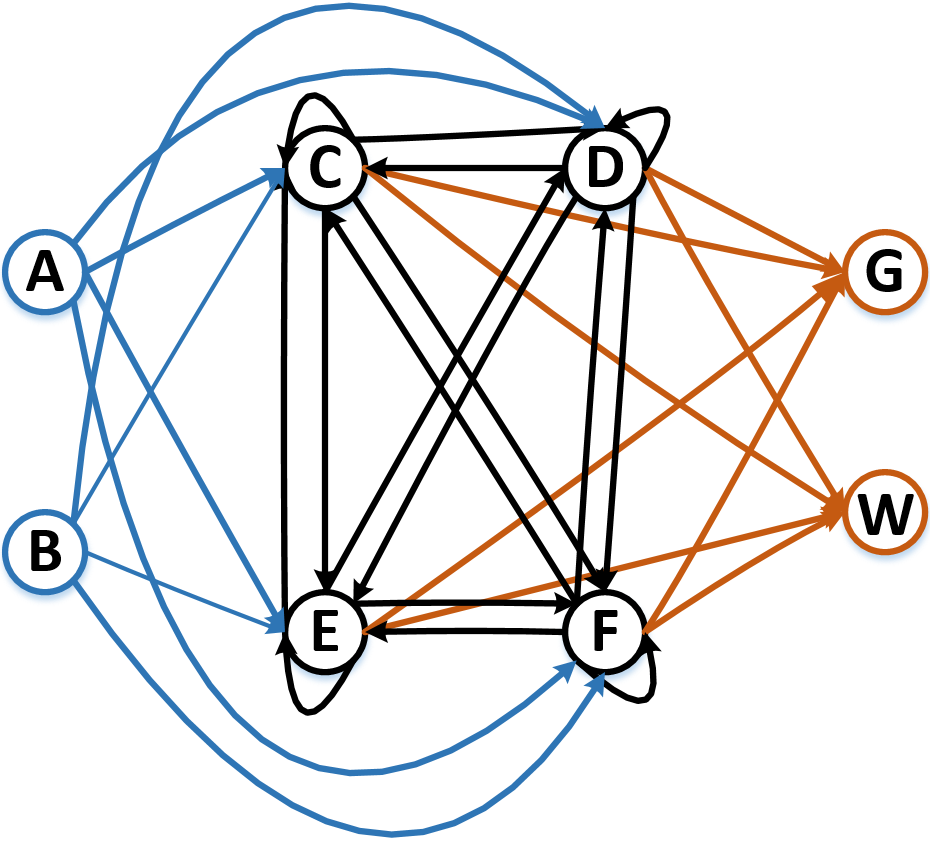
\includegraphics[scale=0.23]{figures/Fig1.png}}
		}}
		
		\caption{A Boolean control network. }%We use blue, black and orange, to distinguish three types of nodes and three types of edges. with two input-nodes $A$ and $B$, four state-nodes $C$, $D$, $E$ and $F$, and two output-nodes $G$, $W$.
		\label{fig:1}
	\end{figure}
%	
Fig.~\ref{fig:1} presents a \BCN\ with two input-nodes $A$ and $B$, four state-nodes $C$, $D$, $E$ and $F$, two output-nodes $G$, $W$. 
The updating rules $f:\mathbb{B}^{6}\mapsto \mathbb{B}^4$ and $h:\mathbb{B}^4\mapsto \mathbb{B}^2$ are given in the truth table (Fig.~\ref{fig:2}) from which the update rule in terms of logic functions can be easily recovered.   For instance, %from the truth table we have 
the updating rule of output-node $G$ is 
$G(t)=C(t)\vee {({D}(t)\wedge { E}(t)\wedge {F}(t))}.$
 \begin{figure}[thpb]
	\centering
	\framebox{\parbox{3in}{
			\centerline{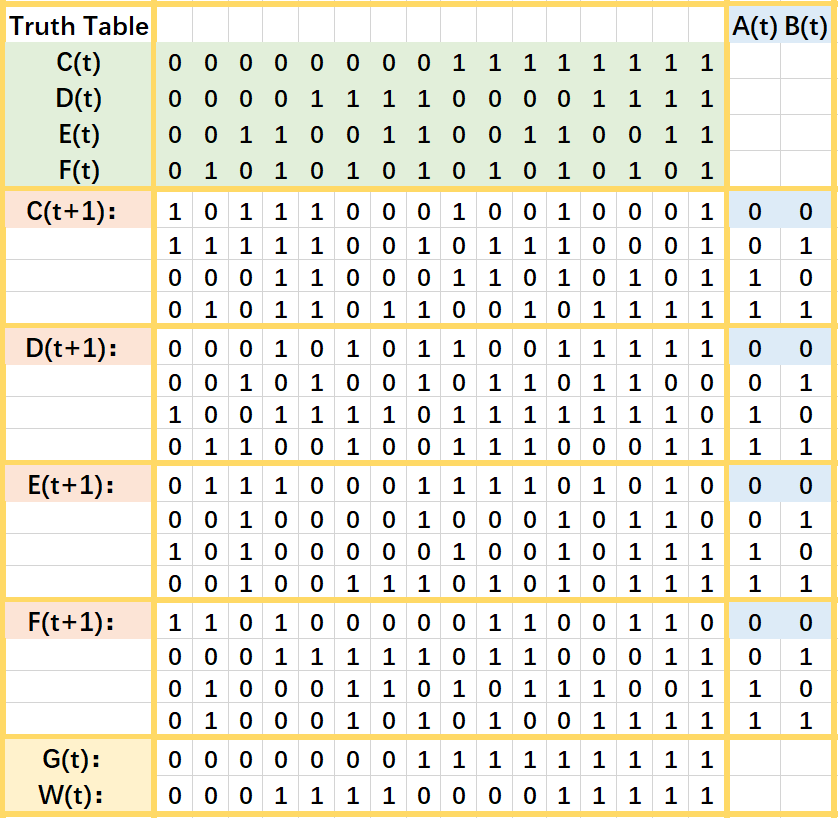
\includegraphics[scale=0.261]{figures/Fig2.png}}
	}}
	\caption{The truth table which describe the updating rules of the \BCN\ shown in Fig.~\ref{fig:1}.}
	\label{fig:2}
\end{figure}
%For instance, from the truth table we have the updating rule of output-node $G$ is 
%$G(t)=C(t)\vee {({D}(t)\wedge { E}(t)\wedge {F}(t))}.$
 %
\end{example}   
%===========================================================

%The reason why we use the truth table to describe the updating rules of the \BCN\ is that it would be more convenient for us to convert the $\mathsf{i}(t)$, $\mathsf{s}(t)$ and $\mathsf{o}(t)$ into their abbreviation forms. 
%That we use 
%\begin{itemize}
%  \item $\delta^i_{2^m}$ represents the abbreviation form of $\mathsf{i}(t)$, where $i=\sum_{x=1}^m \mathsf{i}_{x}(t)\times 2^{m-x}$;
%  \item $\delta^j_{2^n}$ represents the abbreviation form of $\mathsf{s}(t)$, where $j=\sum_{x=1}^n \mathsf{s}_{x}(t)\times 2^{n-x}$;
%  \item $\delta^w_{2^q}$ represents the abbreviation form of $\mathsf{o}(t)$, where  $w=\sum_{x=1}^q \mathsf{o}_{x}(t)\times 2^{q-x}$.
%\end{itemize}
%
%For instance if $\mathsf{s}(t)=\begin{bmatrix}\mathsf{s}_1(t)\\\mathsf{s}_2(t) \\ \mathsf{s}_3(t) \\\mathsf{s}_4(t)\end{bmatrix}=\begin{bmatrix}0\\1\\0\\1\end{bmatrix}$, then $\mathsf{s}(t)$ can be represented by $\delta^{(0\times2^3+1\times2^2+0\times2^1+1\times2^0)}_{2^4}=\delta^5_{16}$. 
%
%In the \BCN\ which shown in the Fig.~\ref{fig:1}, we consider 
%\begin{itemize}
%  \item $A(t)$ as $\mathsf{i}_{1}(t)$, $B(t)$ as $\mathsf{i}_{2}(t)$;
%  \item $C(t)$ as $\mathsf{s}_{1}(t)$, $D(t)$ as $\mathsf{s}_{2}(t)$;
%  \item $E(t)$ as $\mathsf{s}_{3}(t)$, $F(t)$ as $\mathsf{s}_{4}(t)$;
%  \item $G(t)$ as $\mathsf{o}_{1}(t)$, $W(t)$ as $\mathsf{o}_{2}(t)$.
%\end{itemize}
%
%Then, the updating rules which shown in Fig.~\ref{fig:2} can be represented by Fig.~\ref{fig:6}.
% \begin{figure}[thpb]
%      \centering
%      \framebox{\parbox{3in}{
%		\centerline{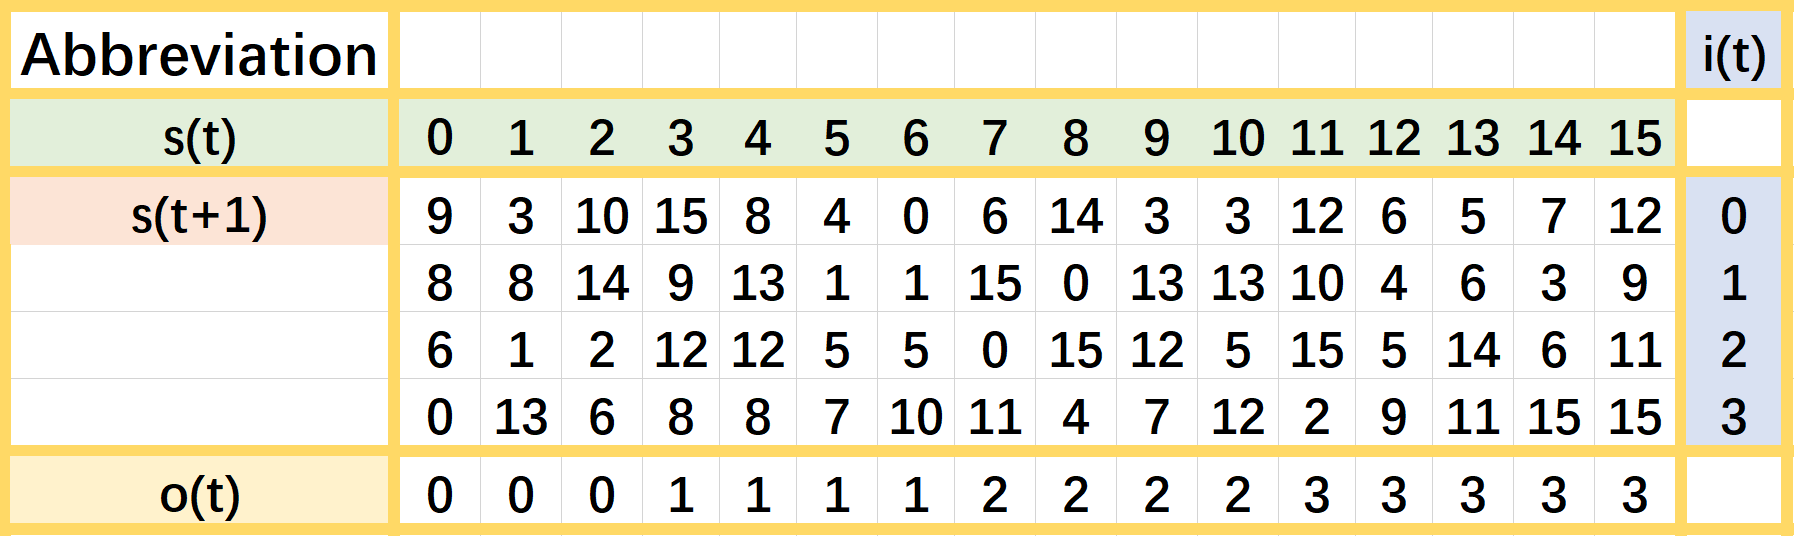
\includegraphics[scale=0.122]{figures/Fig7.png}}
%	}}
%      
%      \caption{The abbreviation form of the updating rules.}
%      \label{fig:6}
%   \end{figure}
%  
%   With the abbreviation forms of $\mathsf{i}(t)$, $\mathsf{s}(t)$ and $\mathsf{o}(t)$, it would be easier for us to use this \BCN\ to explain various concepts by checking this table.
  % 
%For instance, if $\mathsf{s}(t)=\delta^5_{16}$ and $\mathsf{i}(t)=\delta^1_{4}$, then we can know that $\mathsf{s}(t+1)=\delta^4_{16}$  and $\mathsf{s}(t+1)=\delta^1_{4}$ by checking this table.   
  \tl{simplify later?!} 
Moreover, 
   \begin{itemize}
 \item $\Delta_M = \{\delta^0_{2^m},\ldots,\delta^{({2^m}-1)}_{2^m} \}$ represents the input set; 
 \item $\Delta_N = \{\delta^0_{2^n},\ldots,\delta^{({2^n}-1)}_{2^n} \}$ represents the state set; 
 \item $\Delta_Q = \{\delta^0_{2^q},\ldots,\delta^{({2^q}-1)}_{2^q} \}$ represents the output set,
\end{itemize}
where $M=2^m$, $N=2^n$ and $Q=2^q$.
%=======================================================================

%=======================================================================
\subsection{Four existing observability definitions of \BCNs}
In this subsection, we introduce the four existing definitions of observability of \BCNs. 
We first define the mappings \cite{Zhang2016Observability}:
\begin{equation}
\begin{split}
F^k_{\mathsf{s}(t)}:& (\Delta_M)^k\mapsto(\Delta_N)^k\\
&=\mathsf{i}(t)\ldots \mathsf{i}({t+k-1}) \mapsto \mathsf{s}(t+1) \ldots\, \mathsf{s}(t+k)\\
(HF)^k_{\mathsf{s}(0)} :& (\Delta_M)^k\mapsto(\Delta_Q)^k\\
 &=\mathsf{i}(0)\ldots \mathsf{i}(k-1) \mapsto \mathsf{o}(1)\ldots\, \mathsf{o}(k)
\end{split}
\label{equ:6}
\end{equation}
%\tl{but you have defined $\Delta_N$, $\Delta_M$ and $\Delta_Q$ just now?!}
where $\mathsf{s}(t)\in \Delta_N$ and $k>0$. For all  $k>0$,
$\mathsf{I}=\mathsf{i}(t)\ldots \mathsf{i}({t+k-1}) \in(\Delta_M)^k$
is an input sequence, 
$F^k_{\mathsf{s}(t)}(\mathsf{I})=\mathsf{s}(t+1) \ldots\, \mathsf{s}(t+k) \in(\Delta_N)^k$
 is a state sequence, and 
 $(HF)^k_{\mathsf{s}(t)}(\mathsf{I})=\mathsf{o}(t+1)\ldots\, \mathsf{o}(t+k) \in(\Delta_Q)^k$
 is an output sequence. That for every $1\le p \le |\mathsf{I}|$ we have 
 $\mathsf{s}(t+p)=f(\mathsf{i}(t+p-1),\mathsf{s}(t+p-1))$,
and 
 \[\mathsf{o}(t+p)=h(\mathsf{s}(t+p))=h(f(\mathsf{i}(t+p-1),\mathsf{s}(t+p-1))).\] 

%These mappings describe the relations of state ($\mathsf{s}(t)$), input sequence ($\mathsf{I}$), state sequence ($F^k_{\mathsf{s}(t)}(\mathsf{I})$ and $F^{\infty}_{\mathsf{s}(t)}(\mathsf{I})$) and output sequence ($(HF)^k_{\mathsf{s}(t)}(\mathsf{I})$ and $(HF)^{\infty}_{\mathsf{s}(t)}(\mathsf{I})$). 
Then the four existing observability definitions are as follows.

\begin{definition} [First Observability]
The first type of observability is that, a \BCN\ is called observable, if for every initial state \State$^{x}(0)$$\in \Delta_N$, there exists an input sequence $\mathsf{I}^x\in(\Delta_M)^k$ for some $k>0$, such that for all states $\mathsf{s}^{y}(0)\neq \mathsf{s}^{x}(0)$, $h(\mathsf{s}^{y}(0))=h(\mathsf{s}^{x}(0))$ implies $(HF)^k_{\mathsf{s}^{y}(0)}(\mathsf{I}^x)\neq (HF)^k_{{\mathsf{s}^{x}(0)}}(\mathsf{I}^x)$ \cite{cheng2009controllability}.
\end{definition}

The first observability means that a \BCN\ is observable if every \State$^{x}(0)$ of the \BCN\ can be distinguished from other types of initial state by an $\mathsf{I}^x$. Thus, we can only check whether $\mathsf{s}(0)=\mathsf{s}^{x}(0)$ or not by $\mathsf{I}^x$. 
\begin{example}
For example, for the \BCN\ mentioned in {\em Example \ref{exa:2}}, we have every \State$^{x}(0)$ can be distinguished from other types of initial state by an $\mathsf{I}^x \in(\Delta_M)^k$.  For instance,
\begin{itemize}
  \item $\delta_{16}^0$ can be distinguished from other types of initial state by any $\mathsf{I}^0$ with the prefix $\delta_{4}^3$, $\delta_{4}^2$ or $\delta_{4}^0  \delta_{4}^2$;
  \item $\delta_{16}^1$ can be distinguished from other types of initial state by any $\mathsf{I}^1$ with the prefix $\delta_{4}^0$, $\delta_{4}^3$ or $\delta_{4}^2 \delta_{4}^3$;
  \item $\delta_{16}^2$ can be distinguished from other types of initial state by any $\mathsf{I}^2$ with the prefix $\delta_{4}^1$, $\delta_{4}^3$ or $\delta_{4}^0 \delta_{4}^2$, etc.
\end{itemize} 
Therefore this \BCN\ satisfies the first observability.
\label{exa:4}
\end{example}   

\begin{definition}[Second Observability]
	The second type of observability is that, a \BCN\ is called observable if for every two distinct initial states $\mathsf{s}^{x}(0)$, $\mathsf{s}^{y}(0) \in \Delta_N$, there exists an input sequence $\mathsf{I}^{xy}\in(\Delta_M)^k$ for some $k>0$, such that $h(\mathsf{s}^{x}(0))=h(\mathsf{s}^{y}(0))$ implies $(HF)^k_{\mathsf{s}^{x}(0)}(\mathsf{I}^{xy})\neq (HF)^k_{\mathsf{s}^{y}(0)}(\mathsf{I}^{xy})$ \cite{Zhao2010Input}.
\end{definition}

The second observability means that a \BCN\ is called observable if for every two distinct $\mathsf{s}^{x}(0)$, $\mathsf{s}^{y}(0)$, there exists an $\mathsf{I}^{xy}$ which can distinguish them. Therfore, we can only check $\mathsf{s}(0)=\mathsf{s}^{x}(0)$ or $\mathsf{s}(0)=\mathsf{s}^{y}(0)$ when we know that $\mathsf{s}(0)$ is one of them by $\mathsf{I}^{xy}$. 
\begin{example}
For example, for the \BCN\ mentioned in {\em Example \ref{exa:2}}, we have for every two distinct $\mathsf{s}^{x}(0)$ and $\mathsf{s}^{y}(0)$, there exists an $\mathsf{I}^{xy}\in(\Delta_M)^k$ which can distinguish them.  For instance,
\begin{itemize}
  \item $\mathsf{I}^{01}$ with the prefix $\delta_{4}^0$ can distinguish $\delta_{16}^0$ and $\delta_{16}^1$;
  \item $\mathsf{I}^{02}$ with the prefix $\delta_{4}^1$ can distinguish $\delta_{16}^0$ and $\delta_{16}^2$;
  \item $\mathsf{I}^{12}$ with the prefix $\delta_{4}^3$ can distinguish $\delta_{16}^1$ and $\delta_{16}^2$.
\end{itemize} 
Therefore this \BCN\ satisfies the second observability.
\label{exa:5}
\end{example}   
\begin{definition}[Third Observability]
The third type of observability is that, a \BCN\ is called observable if there exists an input sequence $\mathsf{I}\in(\Delta_M)^k$ for some $k>0$, such that for any two distinct states $\mathsf{s}^{x}(0)$, $\mathsf{s}^{y}(0) \in \Delta_N$, $h(\mathsf{s}^{x}(0))=h(\mathsf{s}^{y}(0))$ implies $(HF)^k_{\mathsf{s}^{x}(0)}(\mathsf{I})\neq (HF)^k_{\mathsf{s}^{y}(0)}(\mathsf{I})$ \cite{Cheng2011Identification}.
\end{definition}

The third observability means that a \BCN\ is called observable if there exists an $\mathsf{I}\in(\Delta_M)^k$ which determine the $\mathsf{s}(0)$ of the \BCN\ for every $\mathsf{s}(0)\in\Delta_N$. As $\mathsf{I}$ can distinguish any two distinct $\mathsf{s}^{x}(0)$, $\mathsf{s}^{y}(0)$, the $\mathsf{s}(0)$ is determined by its corresponding output sequence $(HF)^k_{\mathsf{s}(0)}(\mathsf{I})$.

\begin{example}
For example, for the \BCN\ mentioned in {\em Example \ref{exa:2}}, for any $k>0$, there is not any $\mathsf{I}\in(\Delta_M)^k$ which can determine the $\mathsf{s}(0)$ of this \BCN. Because 
\begin{itemize}
  \item any $\mathsf{I}$ with prefix $\delta_{4}^0$ can not distinguish $\delta_{16}^9$ and $\delta_{16}^{10}$;
  \item any $\mathsf{I}$ with prefix $\delta_{4}^1$ can not distinguish $\delta_{16}^0$ and $\delta_{16}^{1}$;
  \item any $\mathsf{I}$ with prefix $\delta_{4}^2$ can not distinguish $\delta_{16}^3$ and $\delta_{16}^{4}$;
  \item any $\mathsf{I}$ with prefix $\delta_{4}^3$ can not distinguish $\delta_{16}^{14}$ and $\delta_{16}^{15}$.
\end{itemize} 
Therefore it does not satisfy the existing third observability, and $\mathsf{s}(0)$ can not be determined. 
\label{exa:6}
\end{example}  
\begin{definition}[Fourth Observability]
	The fourth type of observability is that, \BCN\ is called observable, if there is a $k$ such that for any input sequence $\mathsf{I}\in(\Delta_M)^{k}$, for any two distinct states $\mathsf{s}^{x}(0)$, $\mathsf{s}^{y}(0) \in \Delta_N$, $h(\mathsf{s}^{x}(0))=h(\mathsf{s}^{y}(0))$ implies $(HF)^{k}_{\mathsf{s}^{x}(0)}(\mathsf{I})\neq (HF)^{k}_{\mathsf{s}^{y}(0)}(\mathsf{I})$ \cite{Fornasini2013Observability}.
\end{definition}

The fourth observability means that a \BCN\ is called observable if every sufficient long $\mathsf{I}\in(\Delta_M)^{k}$ can determine the $\mathsf{s}(0)$ of the \BCN\ for every $\mathsf{s}(0)\in\Delta_N$. Because the $\mathsf{I}$ can distinguish any two $\mathsf{s}^{x}(0)$, $\mathsf{s}^{y}(0)$, the $\mathsf{I}$ can be determined by its output sequence $(HF)^k_{\mathsf{s}(0)}(\mathsf{I})$.
\begin{example}
For example, for the \BCN\ mentioned in {\em Example \ref{exa:2}}, we have there exists at least one sufficient long $\mathsf{I}$ that can not determine the $\mathsf{I}$ of this \BCN. For instance, any $\mathsf{I}$ with prefix $\delta_{4}^0$ can not can not distinguish $\delta_{16}^9$ and $\delta_{16}^{10}$. 
Therefore this \BCN\ does not satisfy the fourth observabilityand $\mathsf{s}(0)$ can not be determined either. 
\label{exa:7}
\end{example}  

What is more, we know the implication relationships of four existing types of observability from the definitions of them shown in Fig.~\ref{fig:9}. For the details of the proving process of this proposition, we refer readers to \cite{Zhang2016Observability}.

 \begin{figure}[thpb]
      \centering
      \framebox{\parbox{3in}{
		\centerline{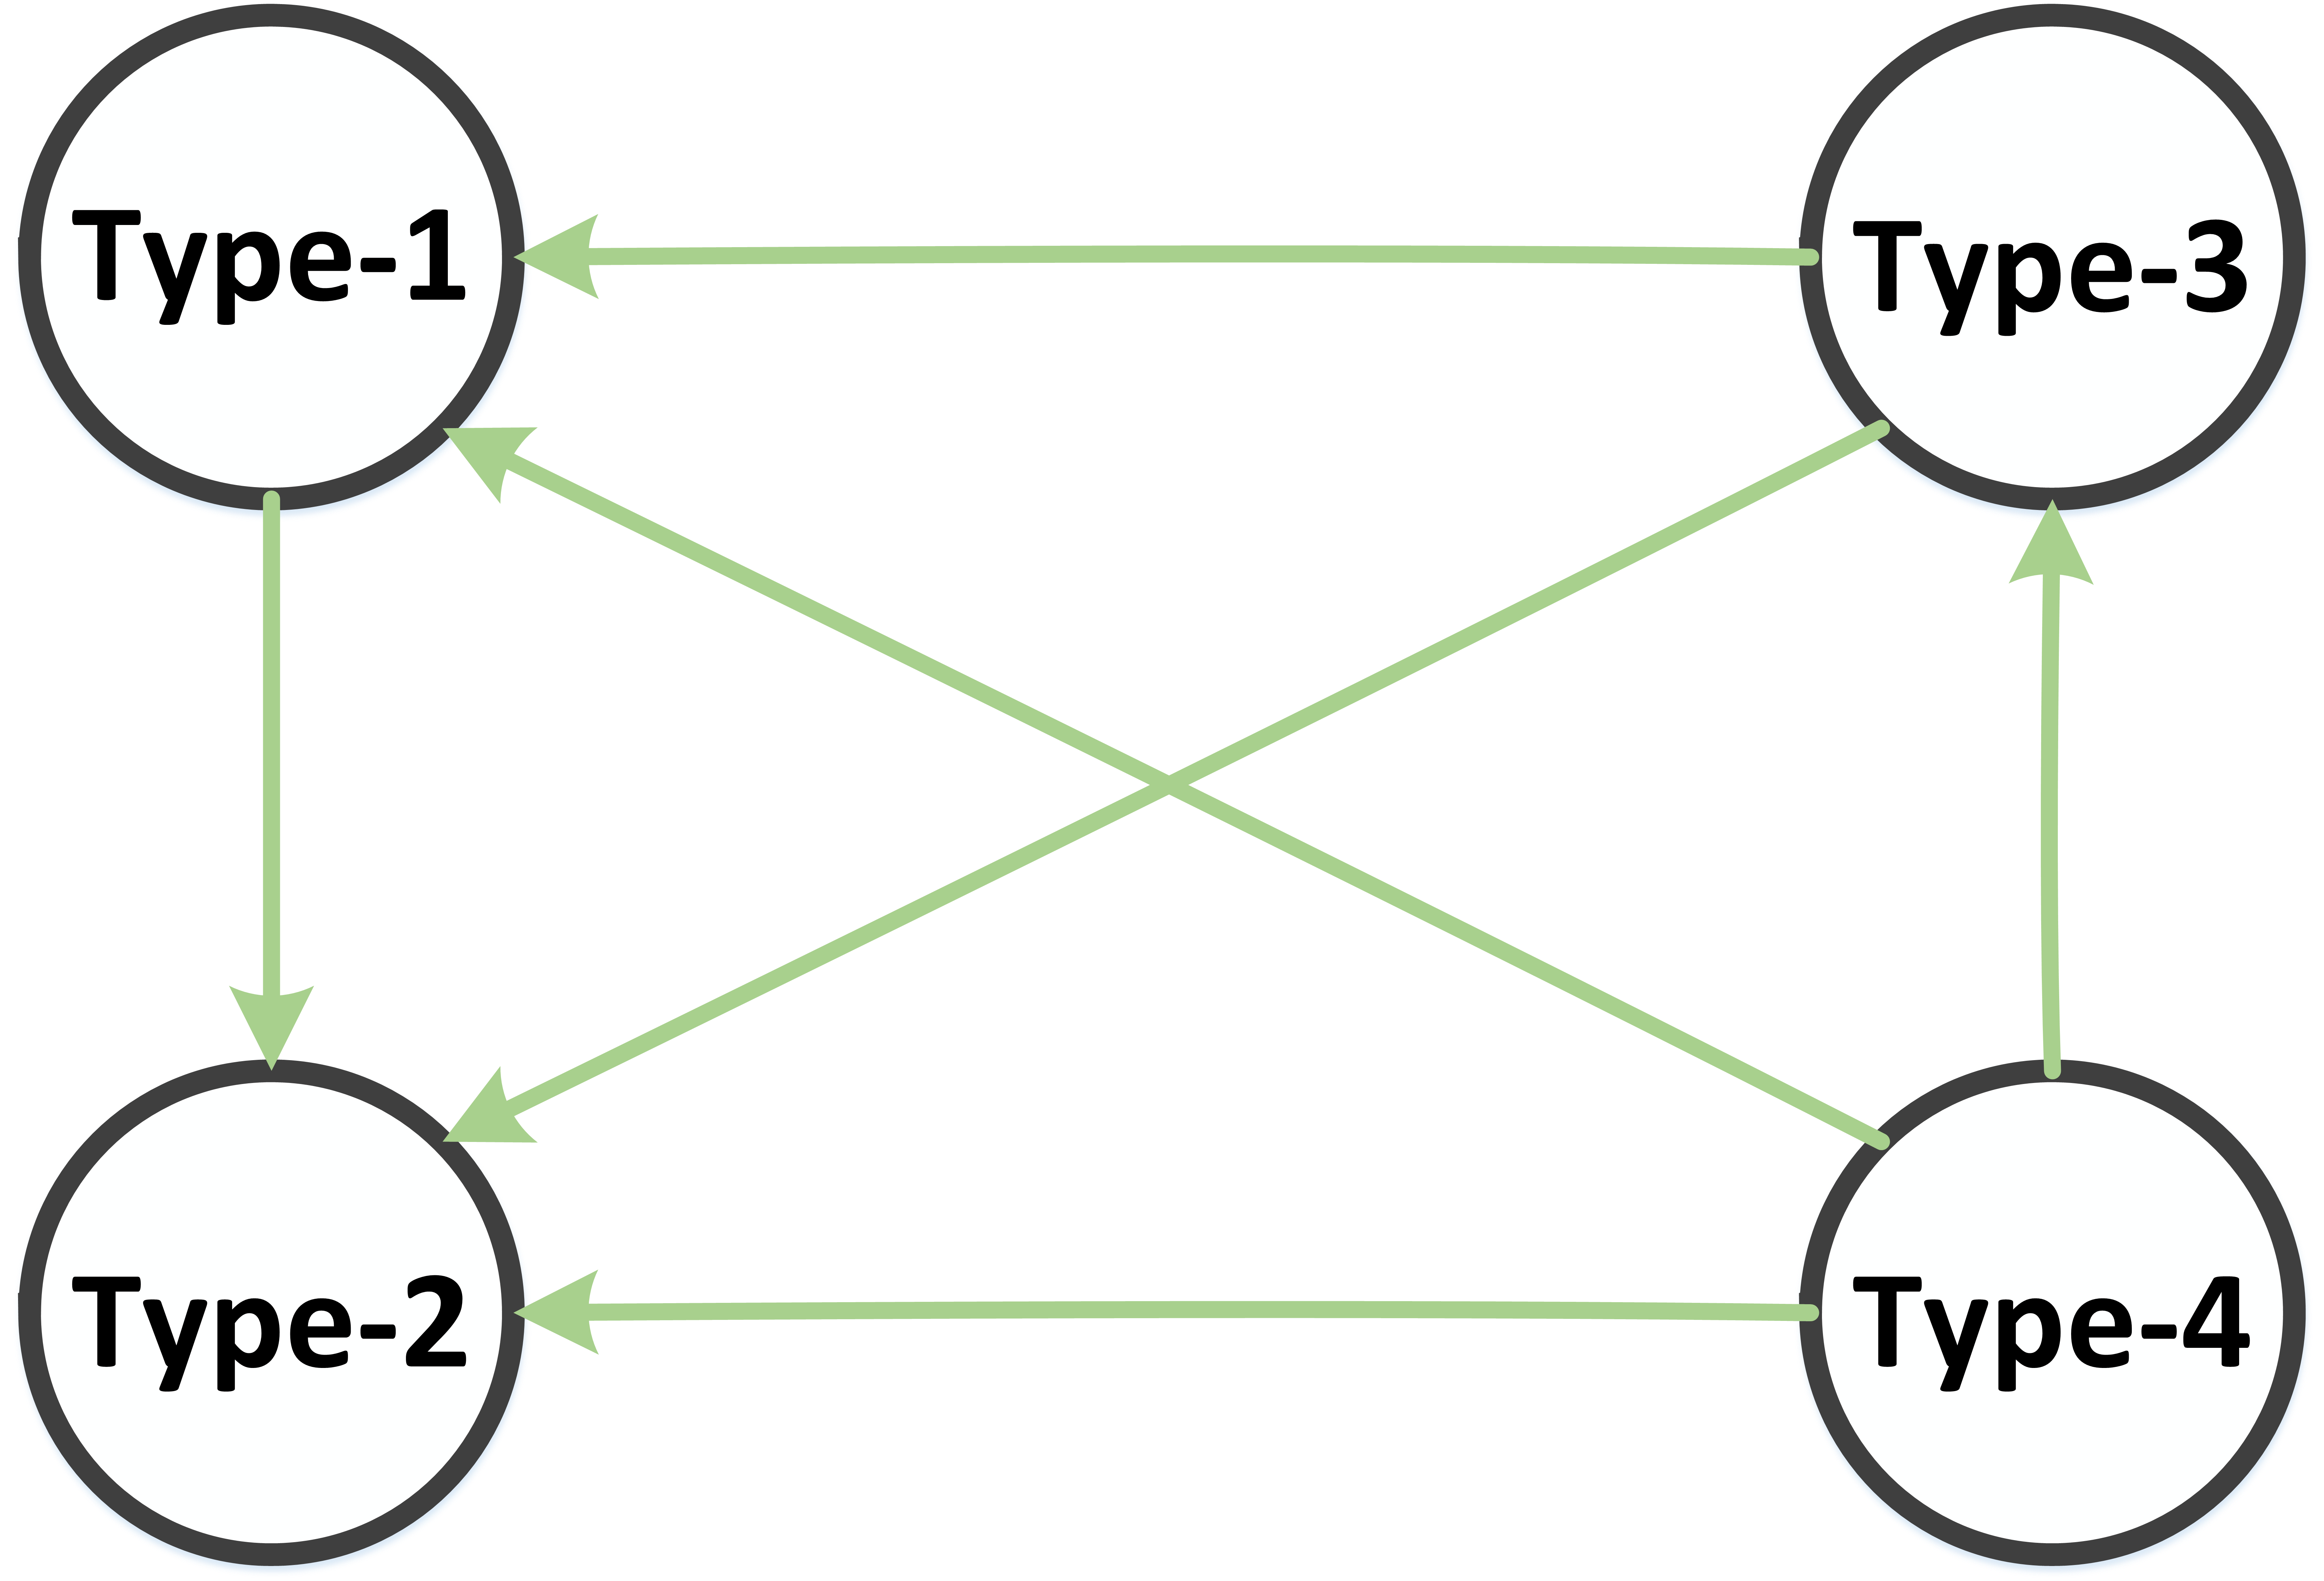
\includegraphics[scale=0.27]{figures/Fig9.png}}
	}}
      
      \caption{The implication relationships graph between existing observability 1, 2, 3, 4, where ``$\rightarrow$" means ``implies".}
      \label{fig:9}
   \end{figure}

%The implication relationship is that ``The first observability implies the second observability.'' means ``If a \BCN\ satisfies the first observability, then it satisfies the second observability.'' 
   
% Because we do not make full use of the output and input in the process of determining the initial state. The output of \BCNs\ we observe at every time step can help us further determine the range of the initial state. With the range of the initial state, we can use different input sequence to determine the initial state. While in the third and fourth existing observability, we use the same input sequence $\mathsf{I}$ to determine the initial state.

 
%However, in some biological systems which depicted by \BCNs, the initial states of them can be checked at most once. Therefore,

As the first observability and second observability are not for determine the initial states of \BCNs. \tl{why this claim?} The third and fourth observability are for determine the initial states of \BCNs, but they are too difficult for \BCNs\ to satisfy. Thus, we propose the online observability of \BCNs\ to solve the problem.
%Moreover, in some biological systems, it would takes many costs to check these biological systems. Hence it would cost a lot of overhead for us to determine the initial state of them by the first observability and second observability.

 \begin{problem}
\label{pro:2}
What is the condition a \BCN\ should satisfy to determine its initial state $\mathsf{s}(0)$ for every $\mathsf{s}(0)\in\Delta_N$?
\end{problem}